\documentclass[addpoints,spanish, 12pt,a4paper]{exam}
%\documentclass[answers, spanish, 12pt,a4paper]{exam}
\printanswers
\pointpoints{punto}{puntos}
\hpword{Puntos:}
\vpword{Puntos:}
\htword{Total}
\vtword{Total}
\hsword{Resultado:}
\hqword{Ejercicio:}
\vqword{Ejercicio:}

\usepackage[utf8]{inputenc}
\usepackage[spanish]{babel}
\usepackage{eurosym}
%\usepackage[spanish,es-lcroman, es-tabla, es-noshorthands]{babel}


\usepackage[margin=1in]{geometry}
\usepackage{amsmath,amssymb}
\usepackage{multicol}
\usepackage{yhmath}

\pointsinrightmargin % Para poner las puntuaciones a la derecha. Se puede cambiar. Si se comenta, sale a la izquierda.
\extrawidth{-2.4cm} %Un poquito más de margen por si ponemos textos largos.
\marginpointname{ \emph{\points}}

\usepackage{graphicx}

\graphicspath{{../img/}} 

\newcommand{\class}{4º Académicas}
\newcommand{\examdate}{\today}
\newcommand{\examnum}{Examen final 2ª evaluación}
\newcommand{\tipo}{A}


\newcommand{\timelimit}{50 minutos}

\renewcommand{\solutiontitle}{\noindent\textbf{Solución:}\enspace}


\pagestyle{head}
\firstpageheader{
\includegraphics[width=0.2\columnwidth]{header_left}}{\textbf{Departamento de Matemáticas\linebreak \class}\linebreak \examnum}{
\includegraphics[width=0.1\columnwidth]{header_right}}
\runningheader{\class}{\examnum}{Página \thepage\ of \numpages}
\runningheadrule

\DeclareUnicodeCharacter{2212}{-}
\begin{document}

\noindent
\begin{tabular*}{\textwidth}{l @{\extracolsep{\fill}} r @{\extracolsep{6pt}} }
\textbf{Nombre:} \makebox[3.5in]{\hrulefill} & \textbf{Fecha:}\makebox[1in]{\hrulefill} \\
 & \\
\textbf{Tiempo: \timelimit} & Tipo: \tipo 
\end{tabular*}
\rule[2ex]{\textwidth}{2pt}
Esta prueba tiene \numquestions\ ejercicios. La puntuación máxima es de \numpoints. 
La nota final de la prueba será la parte proporcional de la puntuación obtenida sobre la puntuación máxima. 

\begin{center}


\addpoints
 %\gradetable[h][questions]
	\pointtable[h][questions]
\end{center}

\noindent
\rule[2ex]{\textwidth}{2pt}

\begin{questions}


% \question[1] 
% \begin{solution} \end{solution}
% \addpoints


\question Resuelve la siguiente inecuación racional:\begin{parts} \part[1] $\dfrac{x^{2} - 4}{x^{2} - 9} \geq  0$\begin{solution} $\left(-\infty, -3\right) \cup \left[-2, 2\right] \cup \left(3, \infty\right)$\end{solution} \part[1] $\dfrac{x^{2} -4x +4}{x^{2} - 1} \geq  0$\begin{solution} $\left(-\infty, -1\right) \cup \left(1, \infty\right)$\end{solution} \part[1] $\dfrac{x^{2} - 4}{x^{2} - 9} \leq  0$\begin{solution} $\left(-3, -2\right] \cup \left[2, 3\right)$\end{solution} \part[1] $\dfrac{x^{2} -2x +1}{x^{2} - 9} \leq  0$\begin{solution} $\left(-3, 3\right)$\end{solution} \end{parts} 


\question Resuelve la siguiente inecuación con valor absoluto:\begin{parts} \part[1] $| {2x - 4} | \leq  8$\begin{solution} $\left[-2, 6\right]$\end{solution} \part[1] $| {2x + 3} | < 5$\begin{solution} $\left(-4, 1\right)$\end{solution} \part[1] $| {3 - 2x} | \leq 7$\begin{solution} $\left[-2, 5\right]$\end{solution} \end{parts} 


\question Resuelve el siguiente sistema de inecuaciones con dos incógnitas:\begin{parts} \part[1] $\left\{\begin{matrix}4x+2y \geq 8 \\ -x+2y < 4\end{matrix}\right.$\begin{solution} \\ \scalebox{.99}{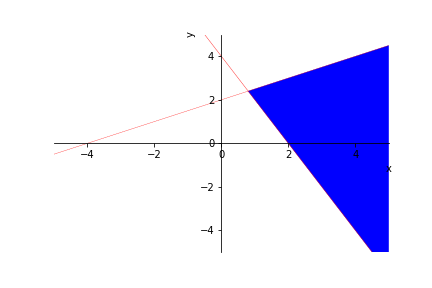
\includegraphics[width=1\columnwidth]{sistema_ine_ex0.png}}\end{solution} \part[1] $\left\{\begin{matrix}2x+y \leq 4 \\ 2x-y > 2 \\ y>-2 \\ x>0\end{matrix}\right.$\begin{solution} \\ \scalebox{.99}{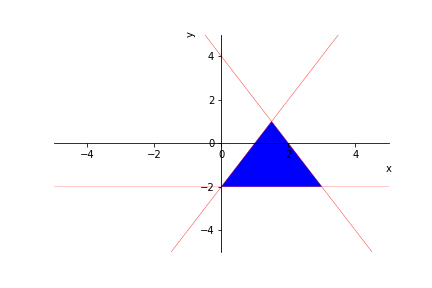
\includegraphics[width=1\columnwidth]{sistema_ine_ex1.png}}\end{solution} \end{parts} 



\question[1] Resuelve por el método que quieras:
$$\left. \begin{gathered}
	  \frac{{x + y}}{2} - \frac{{x - y}}{2} = 2 \hfill \\
	  5x - 10y = 40 \hfill \\ 
	\end{gathered}  \right\rbrace$$
	\begin{solution}  $2y=4 x=\frac{60}{5}=12 \to $x=12; y=2 \end{solution}
	
% \question[1] Resuelve por el método que quieras:
% $$\left. \begin{gathered}
%   \frac{x}{4} + \frac{y}{3} = 2 \hfill \\
%   \frac{x}{8} - \frac{y}{3} = 1 \hfill \\ 
% \end{gathered}  \right\}
% $$
% 	\begin{solution} $\begin{Bmatrix}x : 8, & y : 0\end{Bmatrix}$ \end{solution}

\question Resuelve mediante expresiones algebraicas:
\begin{parts}
\part[2]Juan y su padre se llevan 25 años de edad. Calcular la edad de Juan sabiendo que 
              dentro de 15 años la edad de su padre será el doble que la suya.
          \begin{solution}
              $\left\{\begin{matrix}y=x+25 \\ y+15=2(x+15)\end{matrix}\right. \to  x = 10, \  y = 35$
          \end{solution}
% \part[2] Luisa tiene el triple de edad que su hijo Juan. Dentro de 15 años, la edad de Luisa será el doble que la de su hijo. ¿Cuántos años más que Juan tiene su madre?
% \begin{solution}
%     $\left\{\begin{matrix}y=3x \\ y+15=2(x+15)\end{matrix}\right. \to  x = 15, \  y = 45$
% \end{solution}
% \part[2] La diagonal de un rectángulo mide 2 cm más que uno de los lados. Calcula las dimensiones del rectángulo sabiendo que su perímetro es de 14 cm.
% \begin{solution}
%     $\left\{\begin{matrix}(x+2)^2=x^2+y^2 \\ 2x+2y=14\end{matrix}\right. \to \left[  x = 3, \  y = 4, \   x = 15, \  y = -8\right]$
% \end{solution}
\part[2]  El área de un jardín rectangular mide 900 m2 y está rodeado por un paseo de 5 m de ancho, cuya área es de 850 m2 (la del paseo solo). Calcula las dimensiones del jardín.
\begin{solution}
$\left\{\begin{matrix}xy=900 \\ (x+10)\cdot(y+10)=900+850\end{matrix}\right. \to \left[  x = 15, \  y = 60, \   x = 60, \  y = 15\right]$    
\end{solution}

\end{parts}


\question Resuelve de manera justificada: 
\begin{parts}
% \part[1] $8 x^{2} - 40 x + 48 \geq 0$
% \begin{solution}  $\left(-\infty, 2\right] \cup \left[3, \infty\right)$ \end{solution}
\part[1] $3 x^{2} - 15 x + 18 > 0$
\begin{solution} $\left(-\infty, 2\right) \cup \left(3, \infty\right)$ \end{solution}
% \part[1] $(2 - x)(x - 3)(x - 1)^{2} > 0$
% \begin{solution} $\left(2, 3\right)$ \end{solution}
% \part[1] $(2 - x)(x + 3)(x - 1)^{2} \geq 0$
% \begin{solution} $\left[-3, 2\right]$ \end{solution}
% \part[1] $(2 - x)(x - 3)x^{3} > 0$
% \begin{solution} $\left(-\infty, 0\right) \cup \left(2, 3\right)$ \end{solution}
\part[1] $(2 - x)(x + 3)x^{3} \geq 0$
\begin{solution} $\left(-\infty, -3\right] \cup \left[0, 2\right]$ \end{solution}

\end{parts}

\addpoints

\question Resuelve de manera justificada:
\begin{parts}
\part[2] $\left\{\begin{matrix}\frac{{x - 1}}{2} - \frac{{x + 2}}{3} \leq 12 \\  \frac{x}{2} - \frac{x}{3} \geq 3\end{matrix}\right.$
\begin{solution}
    $\left[18, 79\right]$
\end{solution}
% \part[2] $\left\{\begin{matrix}\frac{{x - 1}}{2} - \frac{{x + 2}}{3} \leq 12 \\  \frac{x}{2} - \frac{x}{3} \leq 1\end{matrix}\right.$
% \begin{solution}
%     $\left(-\infty, 6\right]$
% \end{solution}

\end{parts}

\addpoints

\end{questions}

\end{document}
\grid
